\documentclass[dvisvgm,tikz,border=4pt]{standalone}
\usepackage{amsmath,amssymb}

\usetikzlibrary{arrows.meta,positioning,automata,shapes,shapes.misc,calc,decorations.pathmorphing,decorations.markings,angles,quotes,patterns,mindmap,matrix,knots,hobby,trees}
\tikzset{->-/.style={decoration={markings, mark=at position 0.5 with {\arrow{Stealth}}}, postaction={decorate}}}
\begin{document}
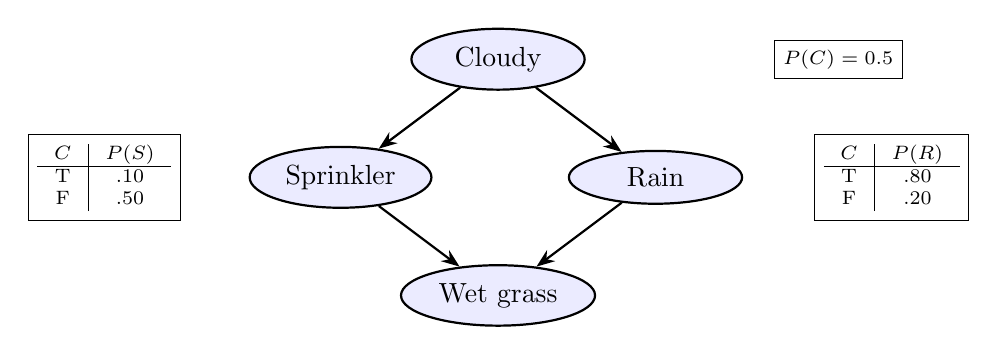
\begin{tikzpicture}[n/.style={ellipse, draw, thick, fill=blue!8, minimum width=2.2cm}, >=Stealth]
\node[n] (c) at (0,2) {Cloudy};
\node[n] (s) at (-2,0.5) {Sprinkler};
\node[n] (r) at (2,0.5) {Rain};
\node[n] (w) at (0,-1) {Wet grass};
\draw[->, thick] (c) -- (s); \draw[->, thick] (c) -- (r); \draw[->, thick] (s) -- (w); \draw[->, thick] (r) -- (w);
\node[draw, font=\scriptsize, align=left, anchor=west] at (3.5,2) {$P(C)=0.5$};
\node[draw, font=\scriptsize] at (-5,0.5) {\begin{tabular}{c|c} $C$ & $P(S)$\\\hline T & .10 \\ F & .50\end{tabular}};
\node[draw, font=\scriptsize] at (5,0.5) {\begin{tabular}{c|c} $C$ & $P(R)$\\\hline T & .80 \\ F & .20\end{tabular}};
\end{tikzpicture}
\end{document}
